\chapter{Environment sensing and perception}\label{chap:environment-sensing-and-perception}

\section*{}

Perception sensors for object recognition have evolved dramatically in the last few years, with the emergence of RGB-D and \gls{tof} sensors (such as the Kinect 1 and 2) as an affordable and reasonably accurate technological solution. Other perception sensors commonly used include 2D and stereo cameras and also camera-laser systems.

\section{Image acquisition}\label{sec:image-acquisition}

With the increase of resolution and lens build quality, 2D sensors remain a viable and accurate solution for detecting objects and perform quality inspection. Moreover, when used to observe the environment from several perspectives, they can achieve good geometry reconstruction and allow accurate 3D perception of objects. The two main image acquisition technologies (\gls{cmos} and \gls{ccd}) are shown in \cref{fig:ccd} and \cref{fig:cmos}.


\begin{figure}[H]
	\begin{floatrow}[2]
		\ffigbox[\FBwidth]
		{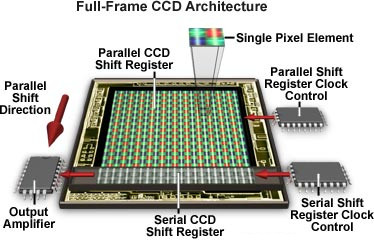
\includegraphics[height=.21\textheight]{sensors/ccd}}
		{\caption[\glsentrytext{ccd} sensor]{\glsentrytext{ccd} sensor\protect\footnotemark}\label{fig:ccd}}

		\ffigbox[\FBwidth]
		{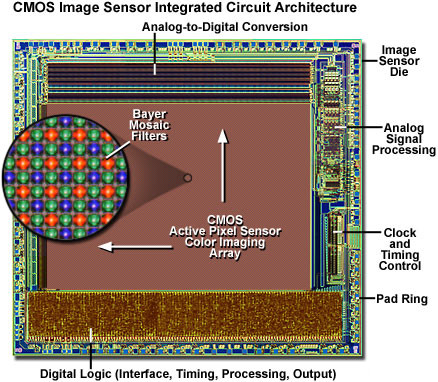
\includegraphics[height=.21\textheight]{sensors/cmos}}
		{\caption[\glsentrytext{cmos} sensor]{\glsentrytext{cmos} sensor\protect\footnotemark}\label{fig:cmos}}
	\end{floatrow}
\end{figure}
\footnotetext[\the\numexpr\value{footnote}-1\relax]{\url{http://cctvsystemblog.blogspot.pt/2013/07/architecture-of-ccd.html}}
\footnotetext[\value{footnote}]{\url{https://micro.magnet.fsu.edu/primer/digitalimaging/cmosimagesensors.html}}


\section{Point cloud acquisition}\label{sec:point-cloud-acquisition}

Point clouds can be retrieved with a wide range of sensors with varying levels of precision and acquisition time \cite{Sansoni2009}. The next sections provide a brief overview of the main technologies capable of generating accurate point clouds useful for 3D perception.


\subsection{Camera-laser systems}

Camera-laser systems can obtain 3D geometry information from the environment by analyzing the deformation pattern of the laser light that is projected into the scene at incremental positions (example in \cref{fig:laser-triangulation}). They can achieve very accurate results, but given the need to physically move the laser or the object to scan, they require longer acquisition periods than the methods presented below.

\begin{figure}[H]
	\centering
	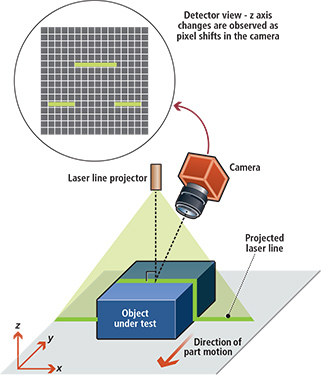
\includegraphics[width=0.4\linewidth]{sensors/laser-triangulation}
	\caption[Camera laser 3D triangulation system]{Camera laser 3D triangulation system\protect\footnotemark}
	\label{fig:laser-triangulation}
\end{figure}
\footnotetext{\url{http://www.vision-systems.com/articles/print/volume-20/issue-6/features/understanding-laser-based-3d-triangulation-methods.html}}


\subsection{Stereo vision methods}

Stereo vision systems (example in \cref{fig:stereo-cameras}) can generate 3D representations of the environment by comparing the displacement of corresponding points in the two ambient images (\cref{fig:stereo-vision} gives an overview of such a system). This can be achieved because the relative position of the cameras is known. As such, points farther away will have smaller displacement between images than points closer to the cameras. In the end, a disparity image is obtained, that can then be converted to a point cloud representation of the environment.

Given that the accuracy of the disparity image relies heavily in the correct matching of points between the left and right image, some stereo vision systems employ active observation by projecting a pattern into the environment in order to refine the point matching (example of hardware setup in \cref{fig:pr2-active-stereo}). This can significantly improve the accuracy if the environment has a lot of smooth surfaces with homogeneous colors.

\begin{figure}[H]
	\begin{floatrow}[2]
		\ffigbox[\FBwidth]
		{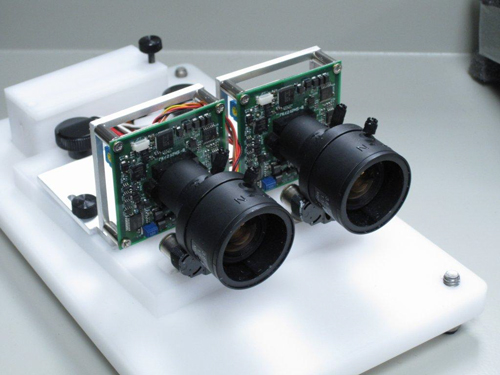
\includegraphics[height=.15\textheight]{sensors/stereo-cameras}}
		{\caption[Stereo vision system]{Stereo vision system \cite{Kaczurba2013}}\label{fig:stereo-cameras}}

		\ffigbox[\FBwidth]
		{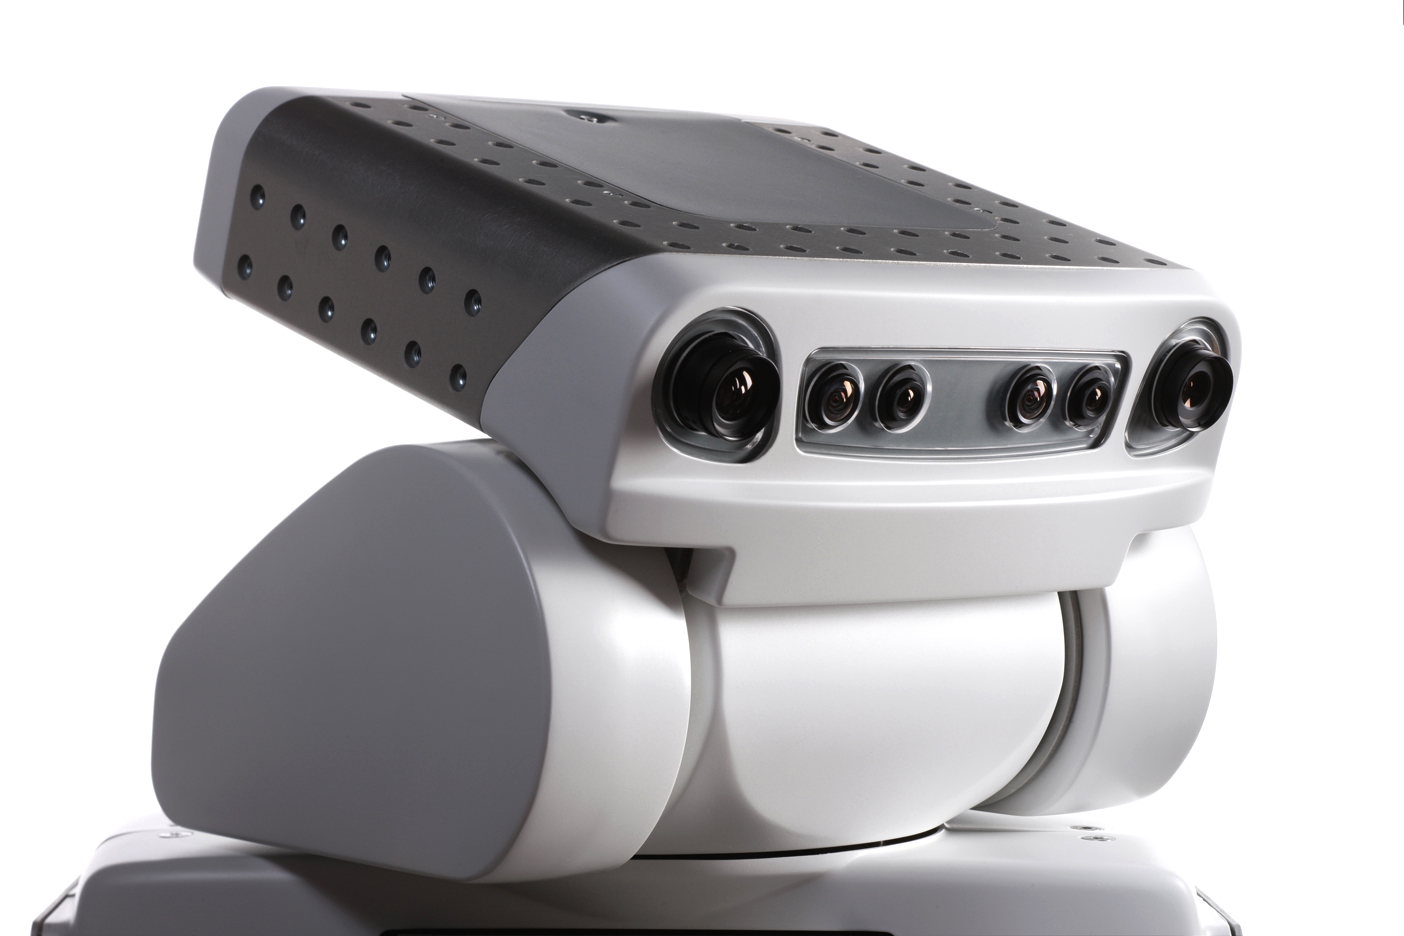
\includegraphics[height=.15\textheight]{sensors/pr2-active-stereo}}
		{\caption[PR2 head capable of active stereo vision]{PR2 head capable of active stereo vision\protect\footnotemark}\label{fig:pr2-active-stereo}}
	\end{floatrow}
\end{figure}
\footnotetext{\url{https://www.willowgarage.com/pages/pr2/overview}}


\begin{figure}[H]
	\centering
	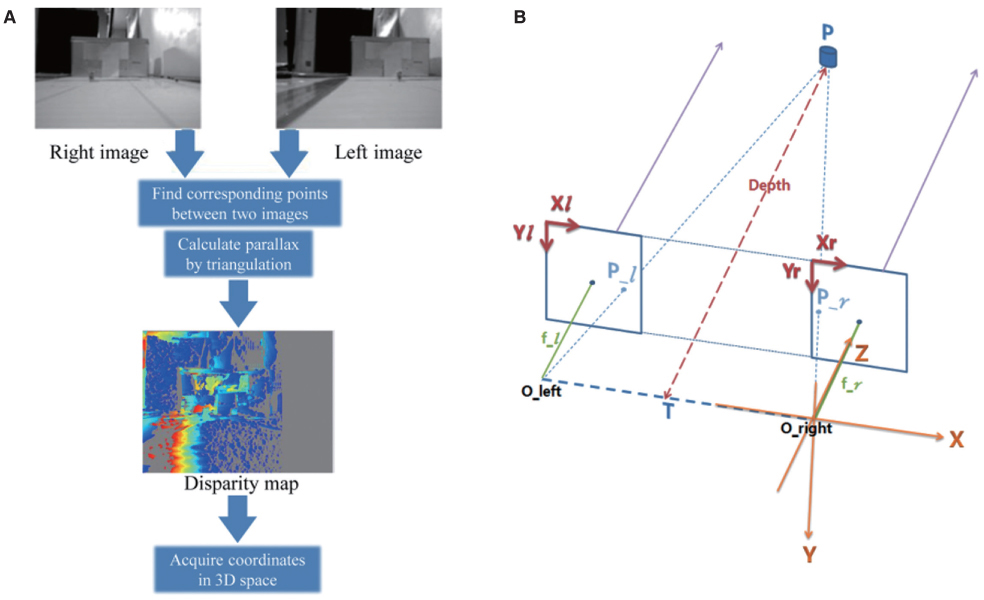
\includegraphics[height=.33\textheight]{sensors/stereo-vision}
	\caption[Stereo vision overview]{Stereo vision overview \cite{Yang2014}}
	\label{fig:stereo-vision}
\end{figure}


\subsection{Structured light methods}

Structured light methods can retrieve 3D geometry from images by projecting a known pattern into the environment and analyzing its deformation (examples in \Cref{fig:structured-light,fig:kinect1-ir}). They can achieve sample rates of 30 Hz and besides 3D geometry they can also retrieve color information.


\begin{figure}[H]
	\begin{floatrow}[2]
		\ffigbox[\FBwidth]
		{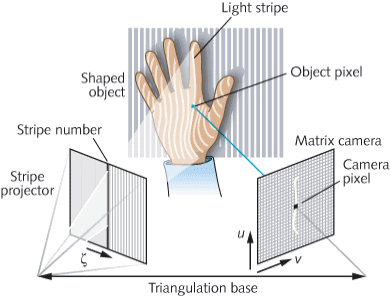
\includegraphics[height=.21\textheight]{sensors/structured-light}}
		{\caption[Structured light system diagram]{Structured light system diagram\protect\footnotemark}\label{fig:structured-light}}

		\ffigbox[\FBwidth]
		{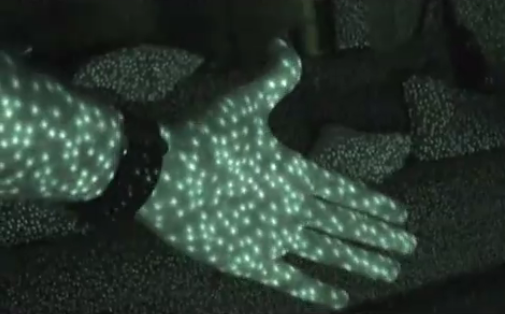
\includegraphics[height=.21\textheight]{sensors/kinect1-ir}}
		{\caption[Kinect 1 \glsentrytext{ir} pattern]{Kinect 1 \glsentrytext{ir} pattern\protect\footnotemark}\label{fig:kinect1-ir}}
	\end{floatrow}
\end{figure}
\footnotetext[\the\numexpr\value{footnote}-1\relax]{\url{http://www.laserfocusworld.com/articles/2011/01/lasers-bring-gesture-recognition-to-the-home.html}}
\footnotetext[\value{footnote}]{\url{https://jahya.net/blog/how-depth-sensor-works-in-5-minutes}}


The Kinect sensor seen in \cref{fig:kinect1} is an example of a structured light system that can achieve measurements with millimeter accuracy for objects close to the sensor. Another similar sensor is the Occipital Structure IO\footnote{\url{http://structure.io/}} which is intended for mobile devices and can be seen in \cref{fig:structure-io}.


\begin{figure}[H]
	\begin{floatrow}[2]
		\ffigbox[1.1\FBwidth]
		{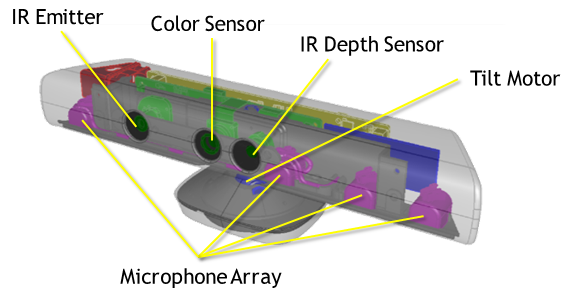
\includegraphics[height=.15\textheight]{sensors/kinect1}}
		{\caption[Kinect 2 sensor]{Kinect sensor\protect\footnotemark}\label{fig:kinect1}}

		\ffigbox[\FBwidth]
		{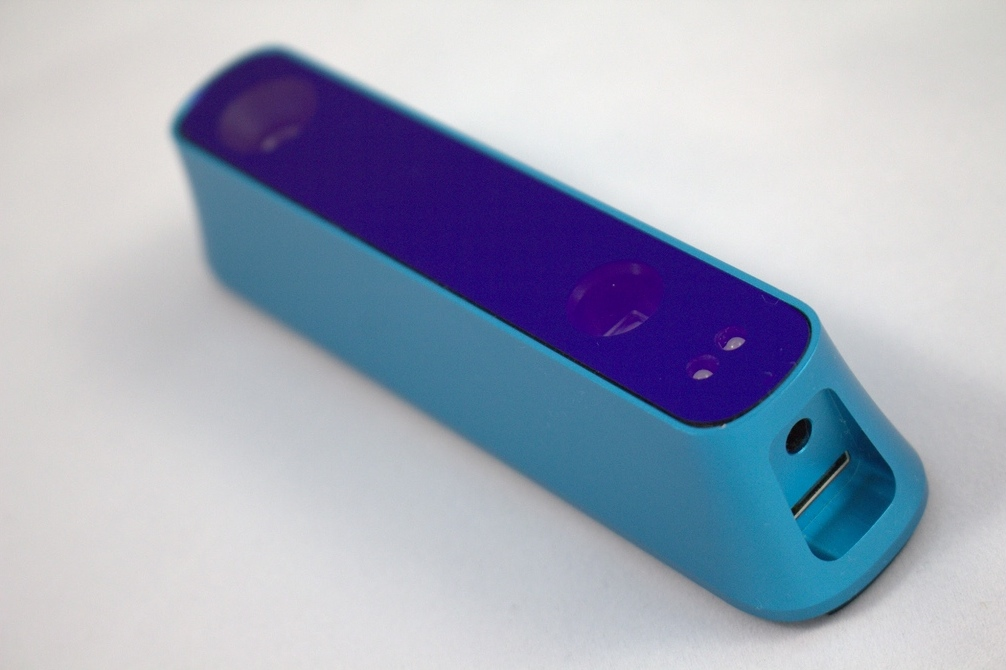
\includegraphics[height=.15\textheight]{sensors/structure-io}}
		{\caption[Structure IO sensor]{Structure IO sensor\protect\footnotemark}\label{fig:structure-io}}
	\end{floatrow}
\end{figure}
\footnotetext[\the\numexpr\value{footnote}-1\relax]{\url{https://msdn.microsoft.com/en-us/library/jj131033.aspx}}
\footnotetext[\value{footnote}]{\url{http://structure.io/press}}


\subsection{\glsentrydesc{tof} methods}\label{sec:tof-methods}

\gls{tof} or \gls{toa} methods can be used to calculate distances based on the amount of time that a given wave takes from the moment it is created to the moment it is received (system operation overview in \cref{fig:time-of-flight}). By acquiring a large amount of sensor readings, a 3D representation of the environment can be achieved.

Since these systems rely on active interaction with the environment, they can be used without being significantly affected by lighting interferences. Nevertheless, it should be taken in consideration the conditions in which the waves propagate and also the geometry of the environment, because it can affect the path that the waves take, and as a result, lead to the decrease of precision in the measurements.


\subsubsection{\glsentrytext{tof} cameras}

\gls{tof} cameras (examples in \cref{fig:mesa-sr4000,fig:kinect2}) can acquire 3D measurements of the environment with very high frame rate (30 Hz or even higher) allowing perception and mapping of the environment with very low latency, which can be a critical requirement in perception tasks that must react very fast to changes in their surroundings.

\begin{figure}[H]
	\centering
	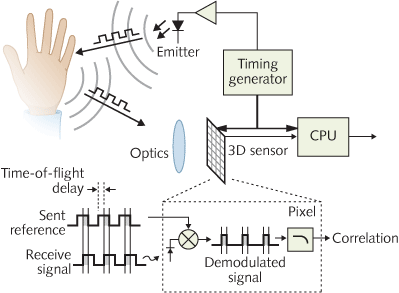
\includegraphics[width=0.6\linewidth]{sensors/time-of-flight}
	\caption[\glsentrydesc{tof} system diagram]{\glsentrydesc{tof} system diagram\protect\footnotemark}
	\label{fig:time-of-flight}
\end{figure}
\footnotetext{\url{http://www.laserfocusworld.com/articles/2011/01/lasers-bring-gesture-recognition-to-the-home.html}}

\begin{figure}[H]
	\begin{floatrow}[2]
		\ffigbox[1.05\FBwidth]
		{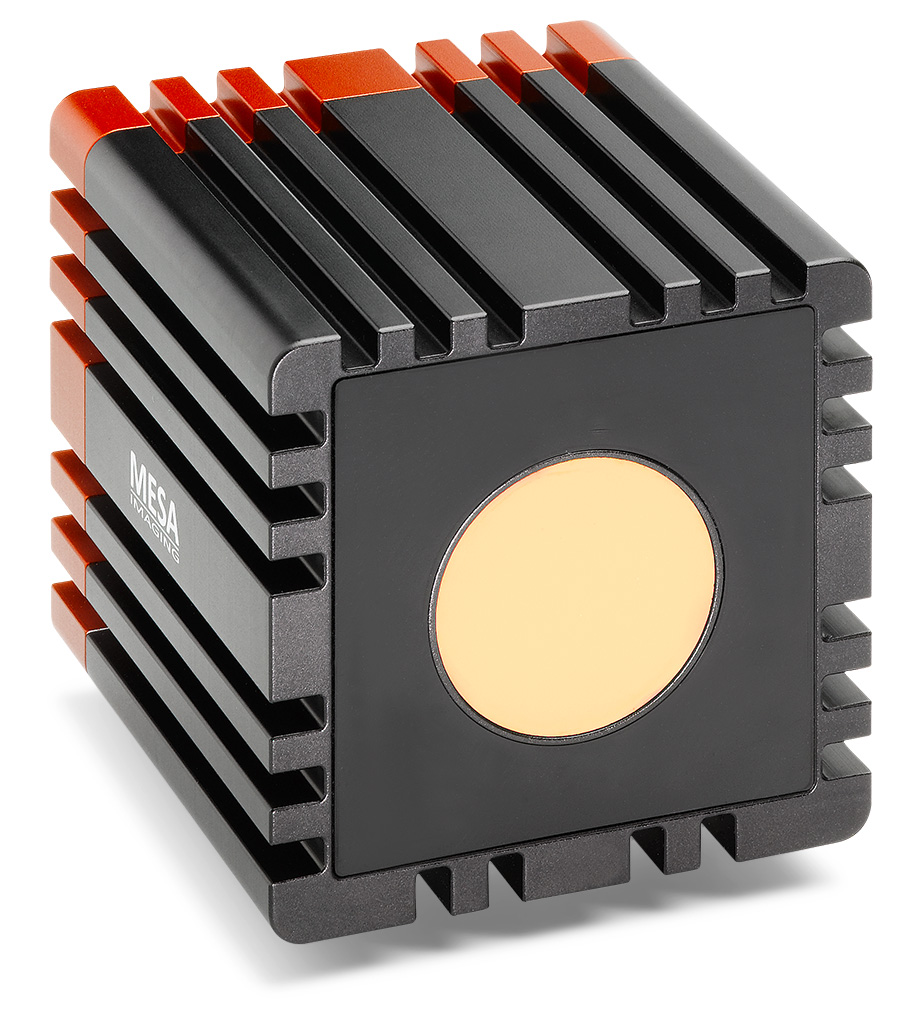
\includegraphics[height=.16\textheight]{sensors/mesa-sr4000}}
		{\caption[Mesa SR4000 sensor]{Mesa SR4000 sensor\protect\footnotemark}\label{fig:mesa-sr4000}}

		\ffigbox[1.05\FBwidth]
		{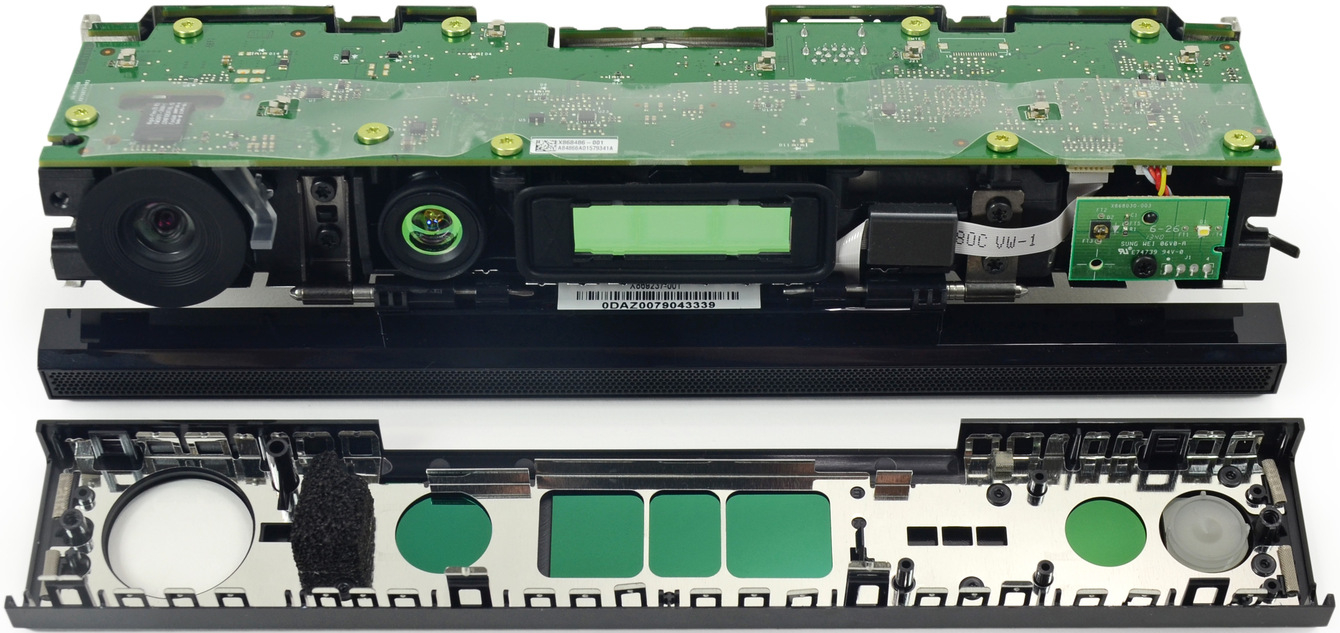
\includegraphics[height=.16\textheight]{sensors/kinect2}}
		{\caption[Kinect 2 sensor]{Kinect 2 sensor\protect\footnotemark}\label{fig:kinect2}}
	\end{floatrow}
\end{figure}
\footnotetext[\the\numexpr\value{footnote}-1\relax]{\url{http://www.mesa-imaging.ch/products/product-overview}}
\footnotetext[\value{footnote}]{\url{https://www.ifixit.com/Teardown/Xbox+One+Kinect+Teardown/19725}}


\subsubsection{\glsentrytext{lidar}}

Light waves generated with lasers can estimate distances with millimeter accuracy at long ranges and their sensors usually have a low sample rate (below 20 Hz). Systems like \gls{lidar} (3D sensor example shown in \cref{fig:velodyne-hdl-64e}) take advantage of this fact and can be used to obtain a very detailed 3D point cloud of the environment (like the one showed in \cref{fig:lidar-scan}). Moreover, some \glspl{lidar} can also capture the environment reflectivity / intensity besides their 3D geometry.

\begin{figure}[H]
	\begin{floatrow}[2]
		\ffigbox[]
		{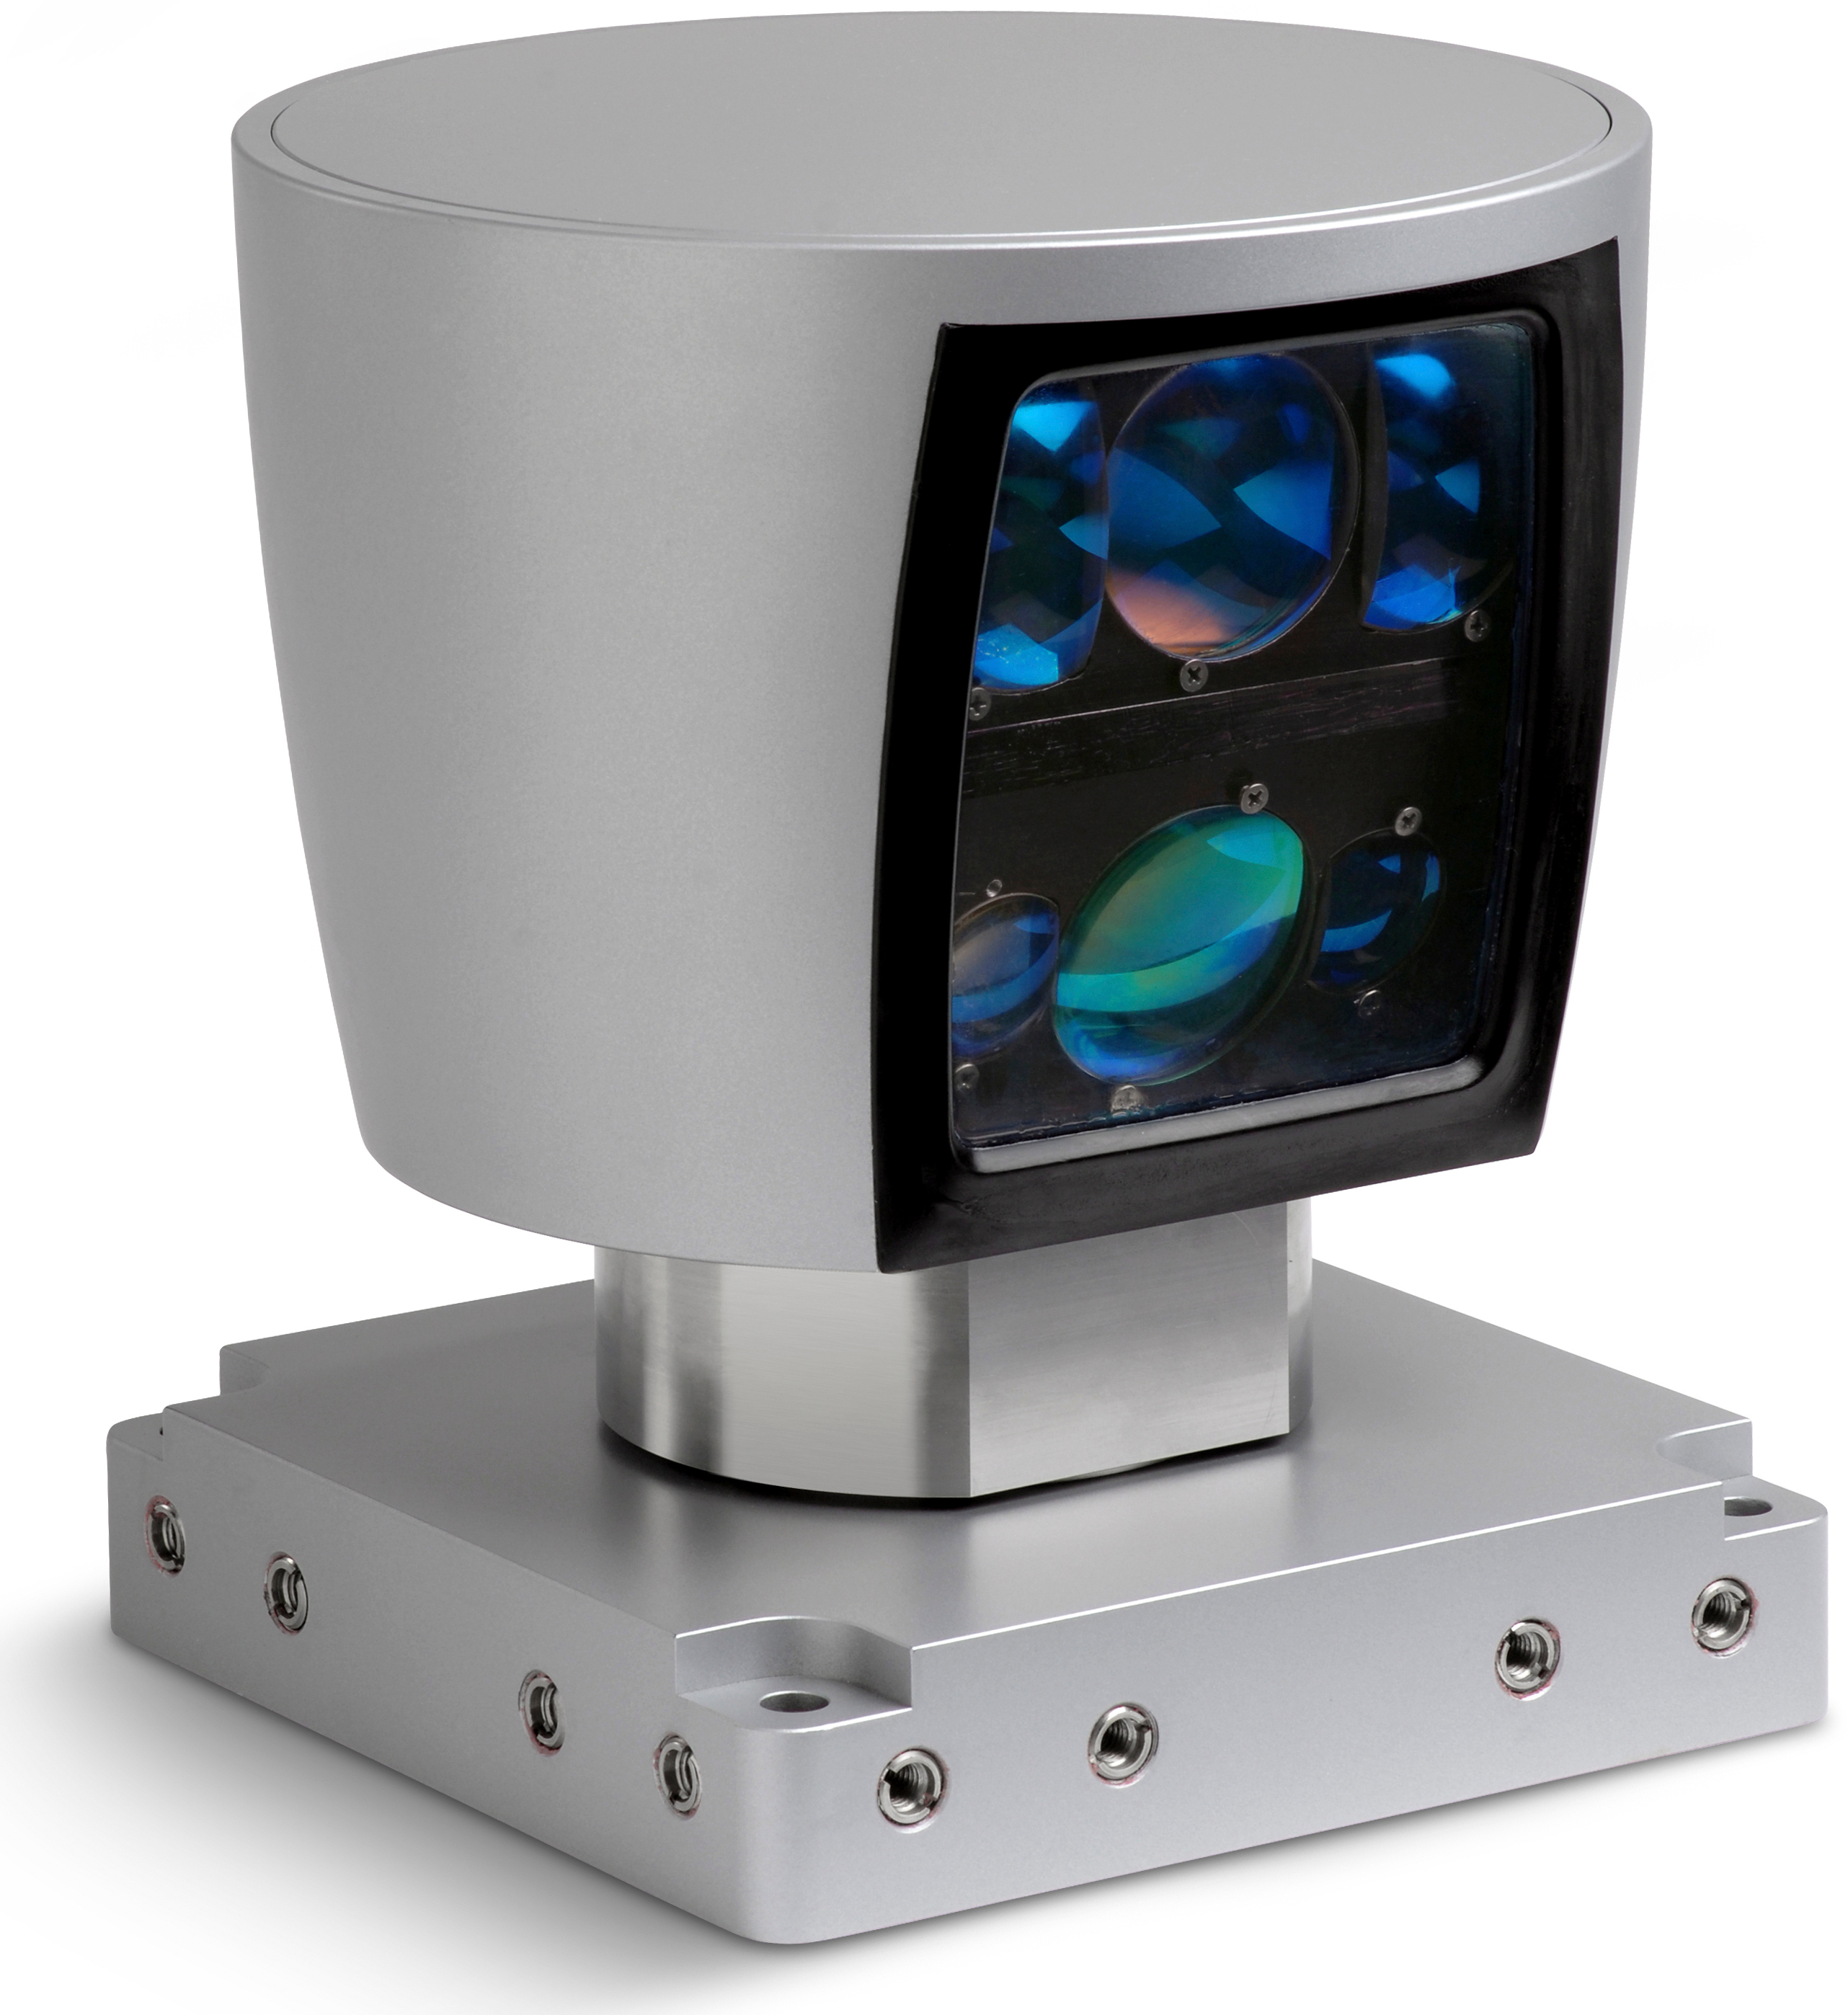
\includegraphics[height=.115\textheight]{sensors/velodyne-hdl-64e}}
		{\caption[3D Velodyne HDL-64E]{3D Velodyne HDL-64E\protect\footnotemark}\label{fig:velodyne-hdl-64e}}

		\ffigbox[]
		{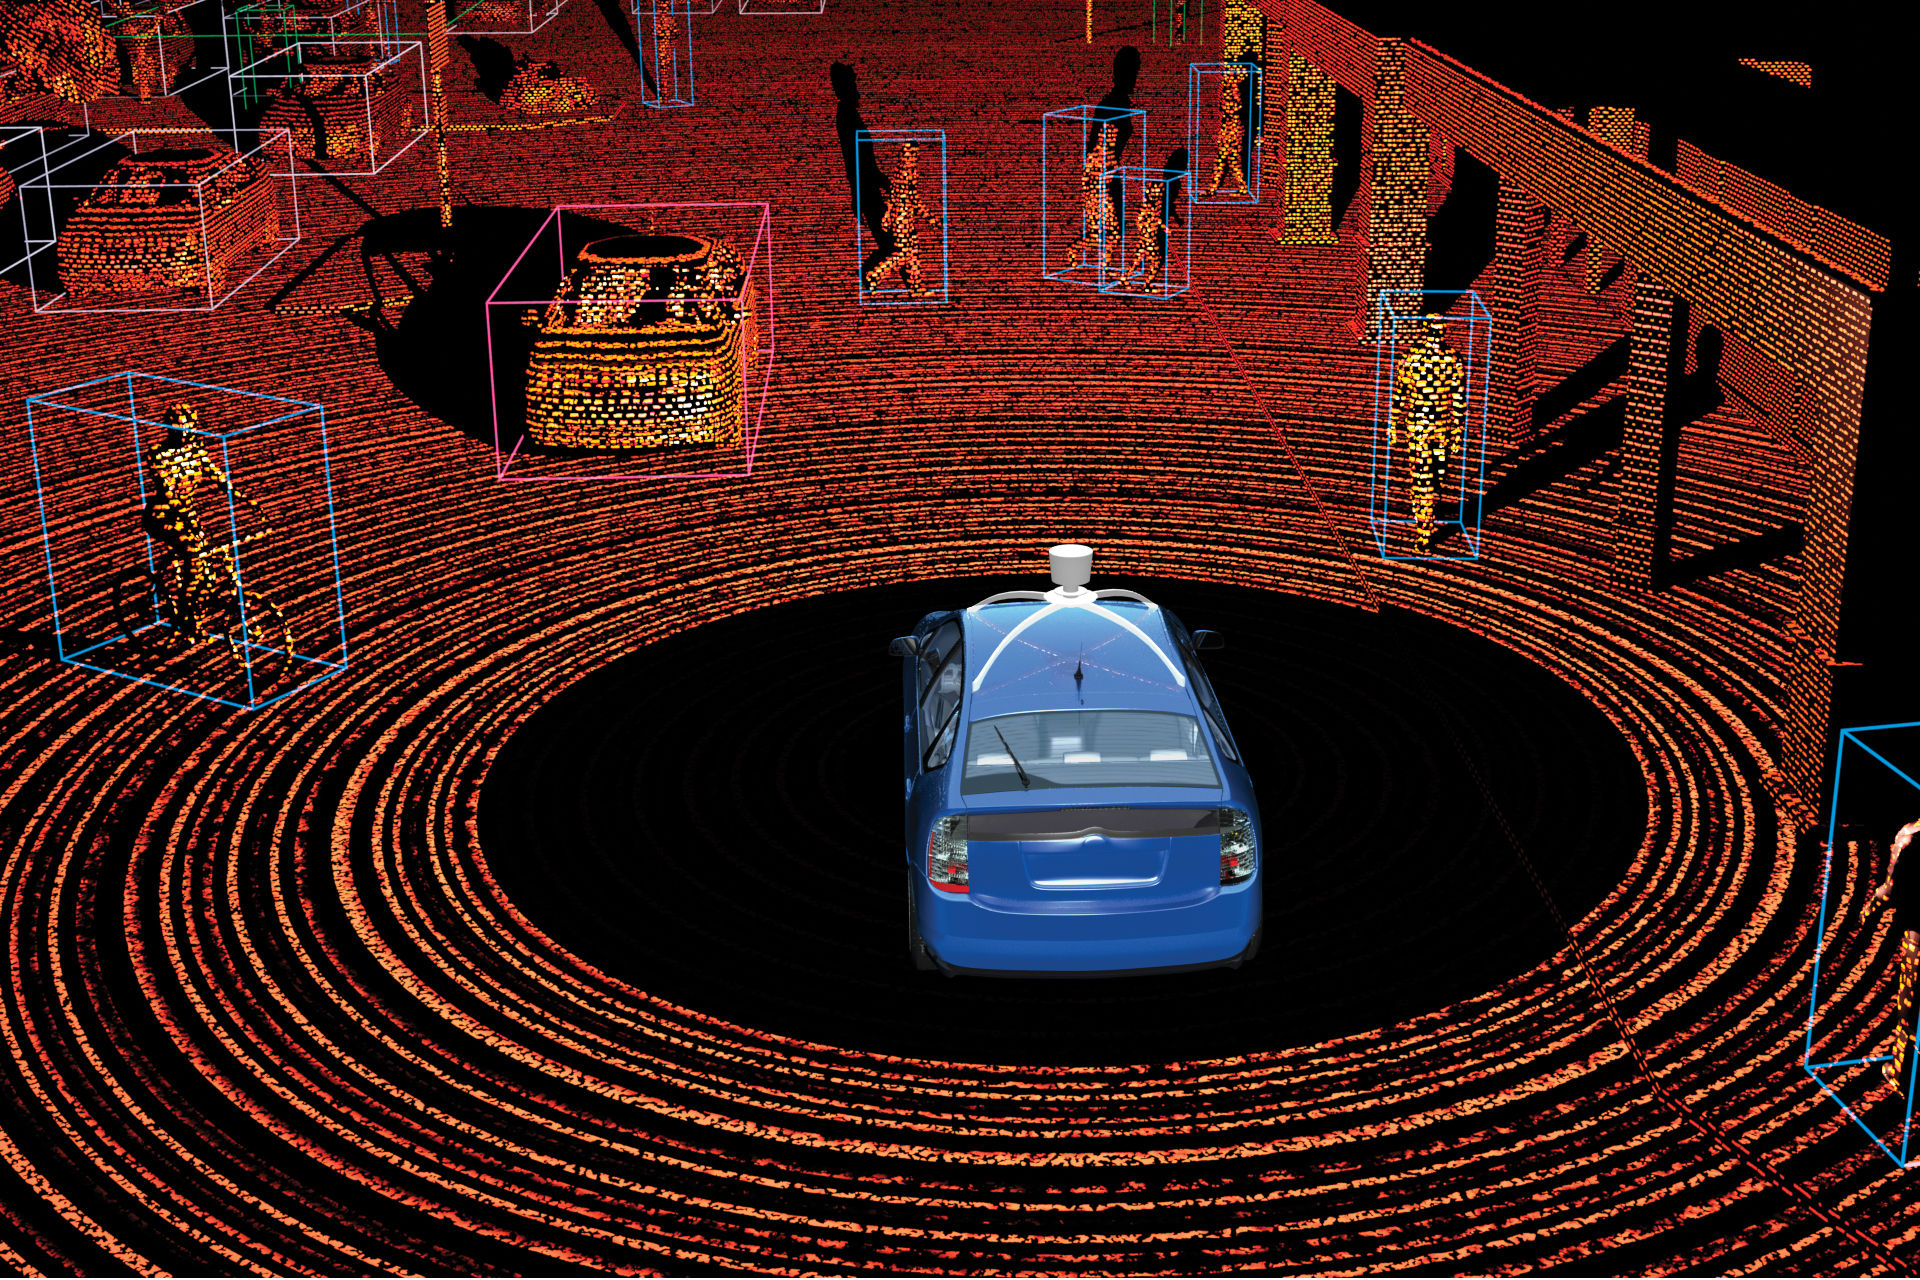
\includegraphics[height=.115\textheight]{sensors/lidar-scan-car}}
		{\caption[\glsentrytext{lidar} scan]{\glsentrytext{lidar} scan\protect\footnotemark}\label{fig:lidar-scan}}
	\end{floatrow}
\end{figure}
\footnotetext[\the\numexpr\value{footnote}-1\relax]{\url{http://www.velodynelidar.com/lidar/hdlproducts/hdl64e.aspx}}
\footnotetext[\value{footnote}]{\url{http://www.popsci.com/cars/article/2013-09/google-self-driving-car}}
